\chapter{Cinematica Inversa}

Prima di iniziare questo capitolo, diamo qualche definizione:
\begin{itemize}
	\item \textbf{Spazio di Lavoro}: Regione descritta dall’origine della terna utensile quando ai giunti del manipolatore si fanno eseguire tutti i movimenti possibili.
	\item \textbf{Spazio di Lavoro Raggiungibile}: Regione dello spazio che l’origine della terna utensile può raggiungere con almeno un orientamento.
	\item \textbf{Spazio di Lavoro Destro}: regione dello spazio che l’origine della terna utensile può raggiungere con più di un orientamento.
	\item \textbf{Spazio Operativo}: Si tratta dello spazio in cui è definito il vettore $\underline{x}$. Questo spazio viene anche chiamato \emph{spazio cartesiano}.
	\item \textbf{Spazio dei Giunti}: Si tratta dello spazio in cui è definito il vettore $\underline{q}$ delle variabili di giunto. Questo spazio viene anche chiamato \emph{spazio delle configurazioni}. 
\end{itemize}

\section{Cinematica diretta e inversa}
\subsubsection{Cinematica Diretta}
Il metodo \emph{D-H} mostra come il problema cinematico diretto $KIN$ sia sempre risolvibile, ovvero, dato un vettore di coordinate di giunto $\underline{q}\in\mathbb{R}^n$, con $q_i$ grandezza lineare di $\theta_i$ (se rotoidale) o di $d_i$ (se prismatico), è sempre possibile calcolare :
\begin{itemize}
	\item la posizione $\underline{p}$ dell'origine della terna utensile (organo terminale)
	\item l'orientazione $R$ della terna utensile rispetto alla terna base
\end{itemize}
queste informazioni sono entrambe contenute nella \emph{matrice di trasformazione omogenea} $T_n^0$ che risulta essere una funzione del vettore $\underline{q}$:
\begin{equation} \label{tensore}
	T_n^0 = T_n^0(\underline{q})
\end{equation}

Nel caso in cui l'orientazione della terna utensile sia specificata in termini di angoli di Eulero (o di un'altra rappresentazione minima dell'orientazione), possiamo definire un vettore $\underline{x}\in\mathbb{R}^n$ che definisce lo \emph{spazio operativo} del robot, come segue:
\begin{equation} \label{posizione_e_orientazione}
	\underline{x} =
	\begin{bmatrix}
		\underline{p} \\
		\phi \\
	\end{bmatrix}
	\quad con \quad
	\underline{\phi} = 
	\begin{bmatrix}
		\varphi \\
		\theta \\
		\psi \\
	\end{bmatrix}
\end{equation}
dove con $\phi$ indico il vettore degli angoli di Eulero che rappresenta l'orientamento dell'organo terminale (terna utensile). 

La cinematica diretta può anche essere scritta come funzione che associa ad un vettore di coordinate di giunto $\underline{q}$ un vettore $\underline{x}$ dello spazio operativo:
\begin{equation}
	\underline{x} = \underline{x}(\underline{q})
\end{equation}

Quindi, la soluzione del problema KIN per meccanismi seriali, formulato come nella \eqref{tensore} oppure come nella \eqref{posizione_e_orientazione} ammette \emph{un'unica soluzione}, pertanto, otteniamo la seguente proposizione:

\paragraph{}
	\emph{Data una certa configurazione del meccanismo, cui è associato un vettore di coordinate di giunto $\underline{q}$, è univocamente determinata la posizione e l'orientazione dell'organo terminale e questa è data, dalla \eqref{tensore} o dalla \eqref{posizione_e_orientazione}}

\subsubsection{Cinematica Inversa}
Il problema cinematico inverso $KIN^{-1}$ consiste nel determinare possibili configurazioni nello \emph{spazio dei giunti} che forniscano una data posizione ed orientazione dell'organo terminale. Non esistono procedure standard per cercare possibili soluzioni.

In pratica, conosciamo $T_n^0$ oppure $\underline{x}$ e vogliamo calcolare delle $n-uple$ $\underline{q}$ tali che:
\begin{equation*}
	\begin{cases}
		\underline{x}(\underline{q}) = \underline{x} \quad assegnata \\
		T_n^0(\underline{q}) = T_n^0 \quad assegnata \\
	\end{cases}
\end{equation*}

Il problema $KIN^{-1}$ risulta più complesso perchè dato un certo meccanismo, possono esistere o meno soluzioni e, se esistono soluzioni, queste possono essere in numero finito o infinito.

Supponiamo di avere una orientazione desiderata $R_{des}$ e una posizione desiderata $\underline{p}_{\,des}$, possono accadere tre cose:
\begin{enumerate}
	\item $R_{des}$, $\underline{p}_{\,des}$ non appartengono allo spazio di lavoro $\Rightarrow$ $0$ soluzioni.
	\item $R_{des}$, $\underline{p}_{\,des}$ appartengono allo spazio di lavoro, ma ci sono infiniti modi di risolvere il problema $\Rightarrow$ $\infty$ soluzioni.
	\item $R_{des}$, $\underline{p}_{\,des}$ appartengono allo spazio di lavoro e vi è un numero preciso di soluzioni del problema $\Rightarrow$ $\exists$ un numero finito di soluzioni.
\end{enumerate}
\newpage

\section{Esempi manipolatori planari}
Consideriamo il caso planare, la posizione e l'orientazione dell'organo terminale (pinza) possono essere specificate con tre parametri ($p_x$, $p_y$, $\phi$). Vediamo gli esempi:

\subsubsection{Robot planare 2R}
Un robot seriale 2R (con due giunti rotoidali) può raggiungere la posizione desiderata $\underline{p}$ in due modi possibili: \emph{elbow up} (gomito alto) e \emph{elbow down} (gomito basso). Una volta scelte le coordinate di giunto $q_1$ e $q_2$ in modo da soddisfare la specifica posizionale, l'orientazione dell'organo terminale $\phi$ è fissata e quindi non possiamo scegliere arbitrariamente l'orientazione e pertanto l'orientazione desiderata non è soddisfatta. Notiamo che il punto $\underline{p}$ appartiene allo \emph{spazio di lavoro destro} perchè è raggiungibile con due orientazioni. 

Pertanto la soluzione al problema cinematico inverso è una sola, ovvero, quella disegnata sotto che soddisfa l'orientazione e la posizione. Ma non ne posso trovare altre perchè ruotando i giunti, l'orientazione cambia.

\begin{center}
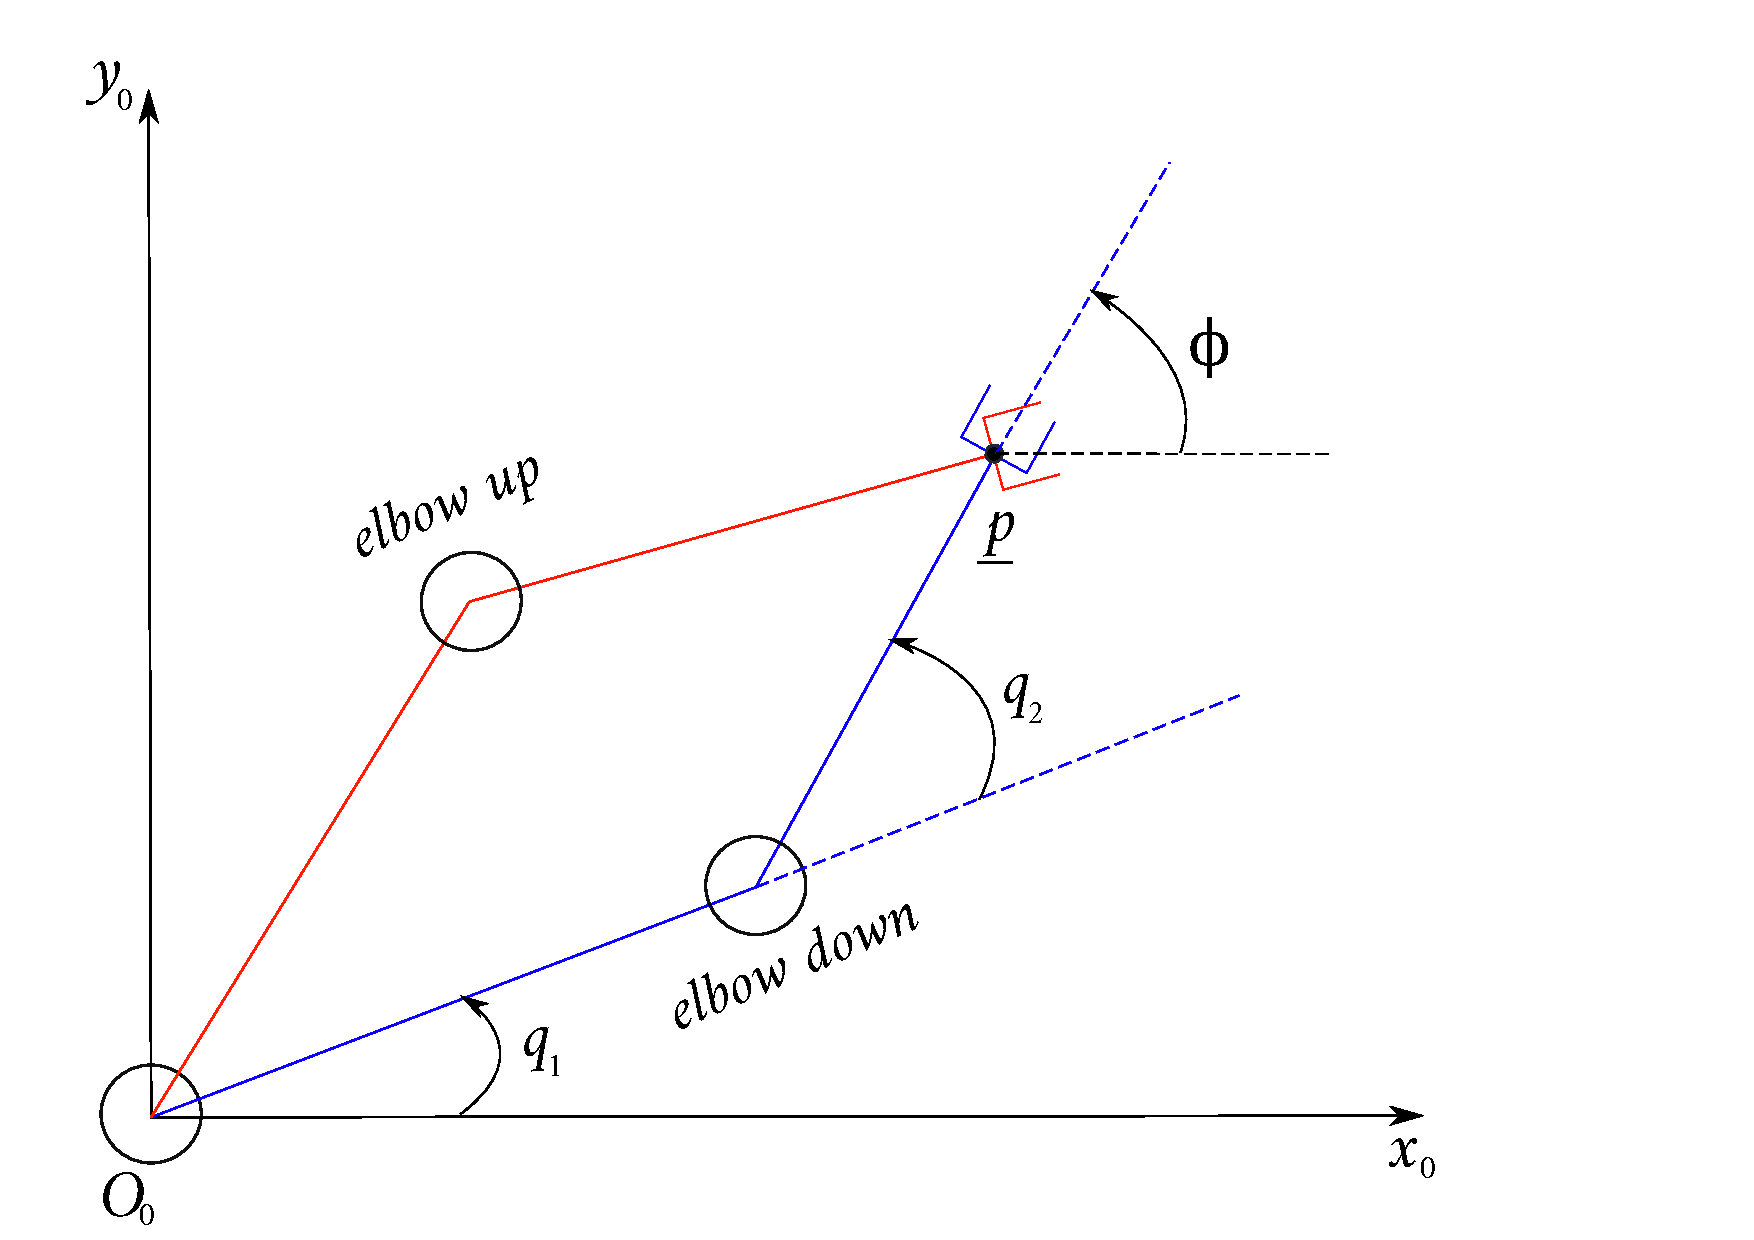
\includegraphics[scale=0.3]{manipolatoreInverso2R.pdf}
\captionof{figure}{Manipolatore planare 2R.}
\end{center}

\subsubsection{Robot planare 3R}
In un robot planare 3R è possibile soddisfare sia la specifica posizionale che la specifica dell'orientazione. Le soluzioni possibili sono due.

\begin{center}
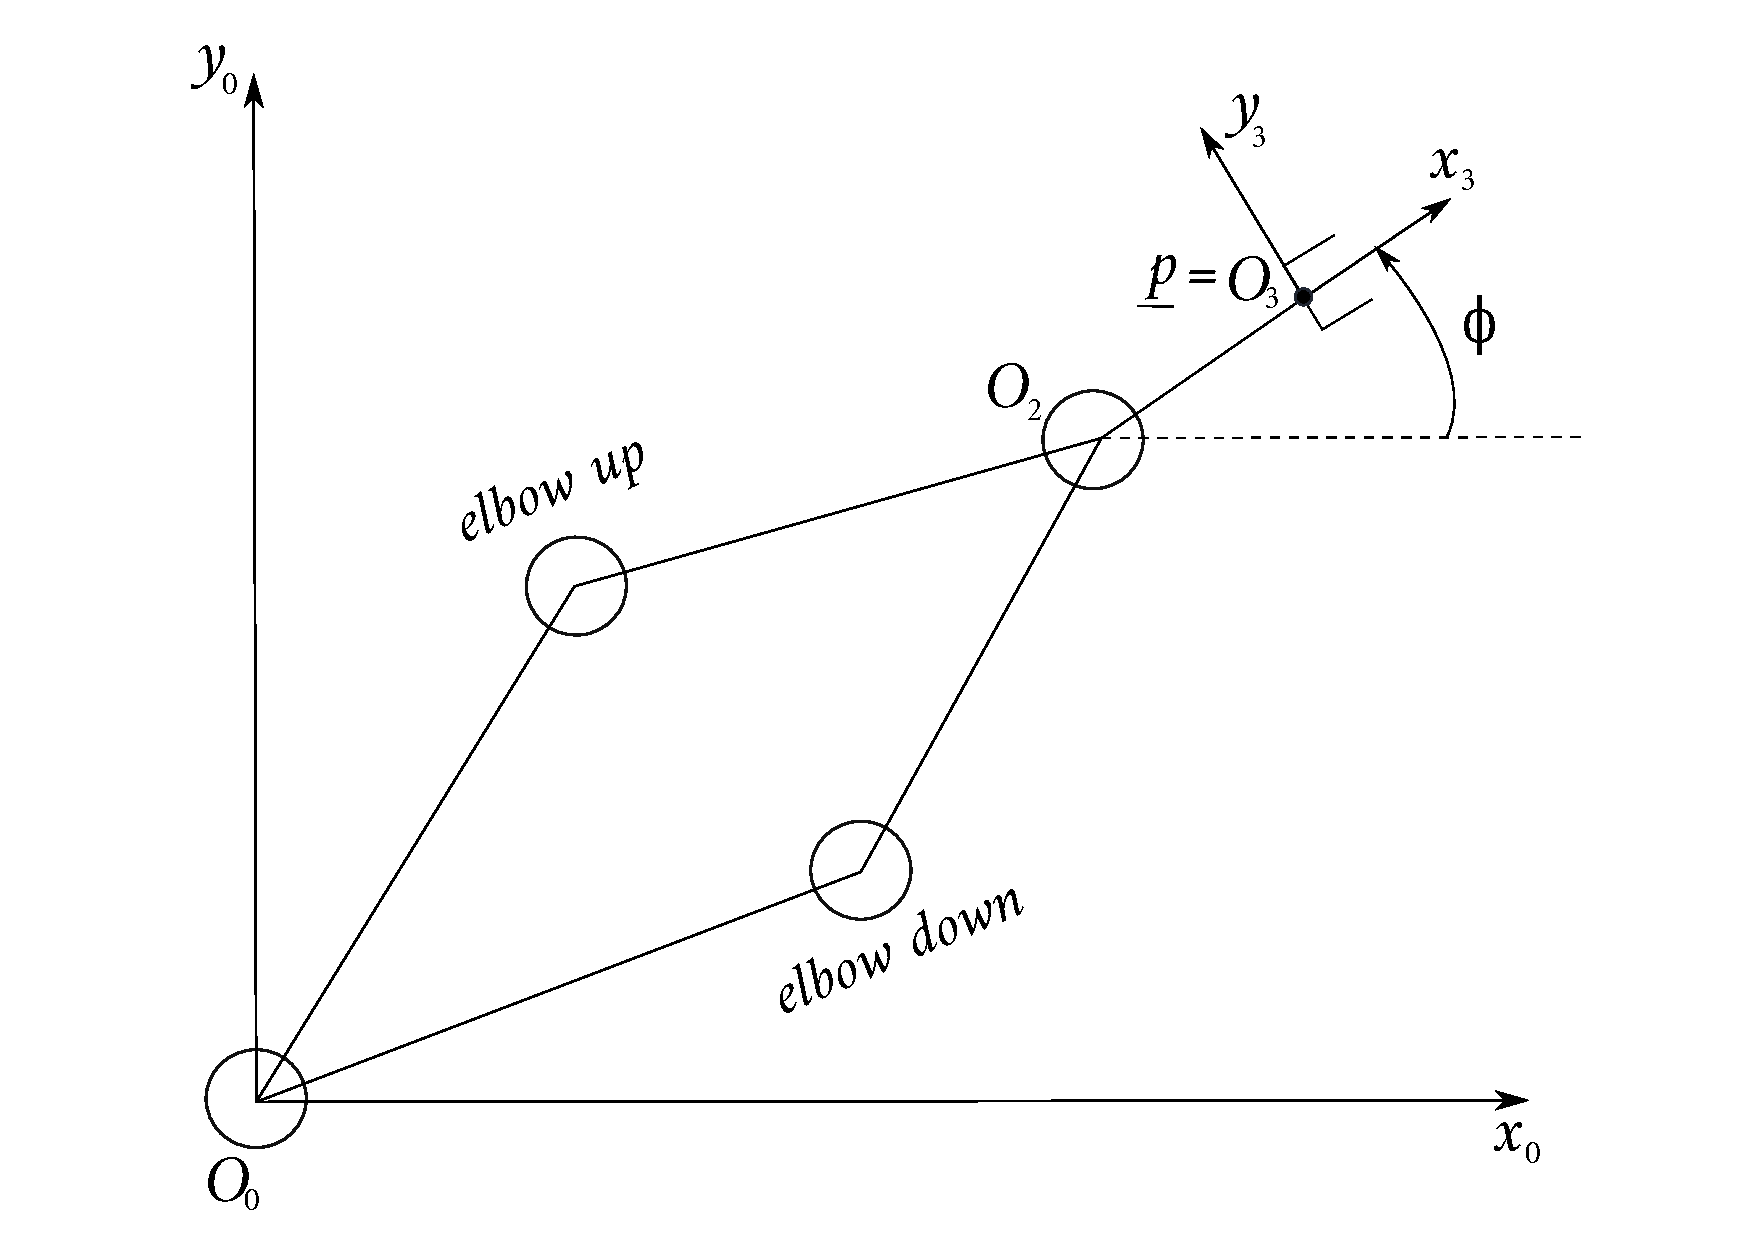
\includegraphics[scale=0.3]{manipolatoreInverso3R.pdf}
\captionof{figure}{Manipolatore planare 3R.}
\end{center}

Troviamo $\underline{q} = [q_1 \; q_2 \; q_3]^T$ che soddisfa la specifica di posa $\underline{p}$, $\phi$. Semplifichiamo il problema eliminando la terza coordinata posizionale e consideriamo $\underline{w}$ come in figura ($3.3$a).

\begin{center}
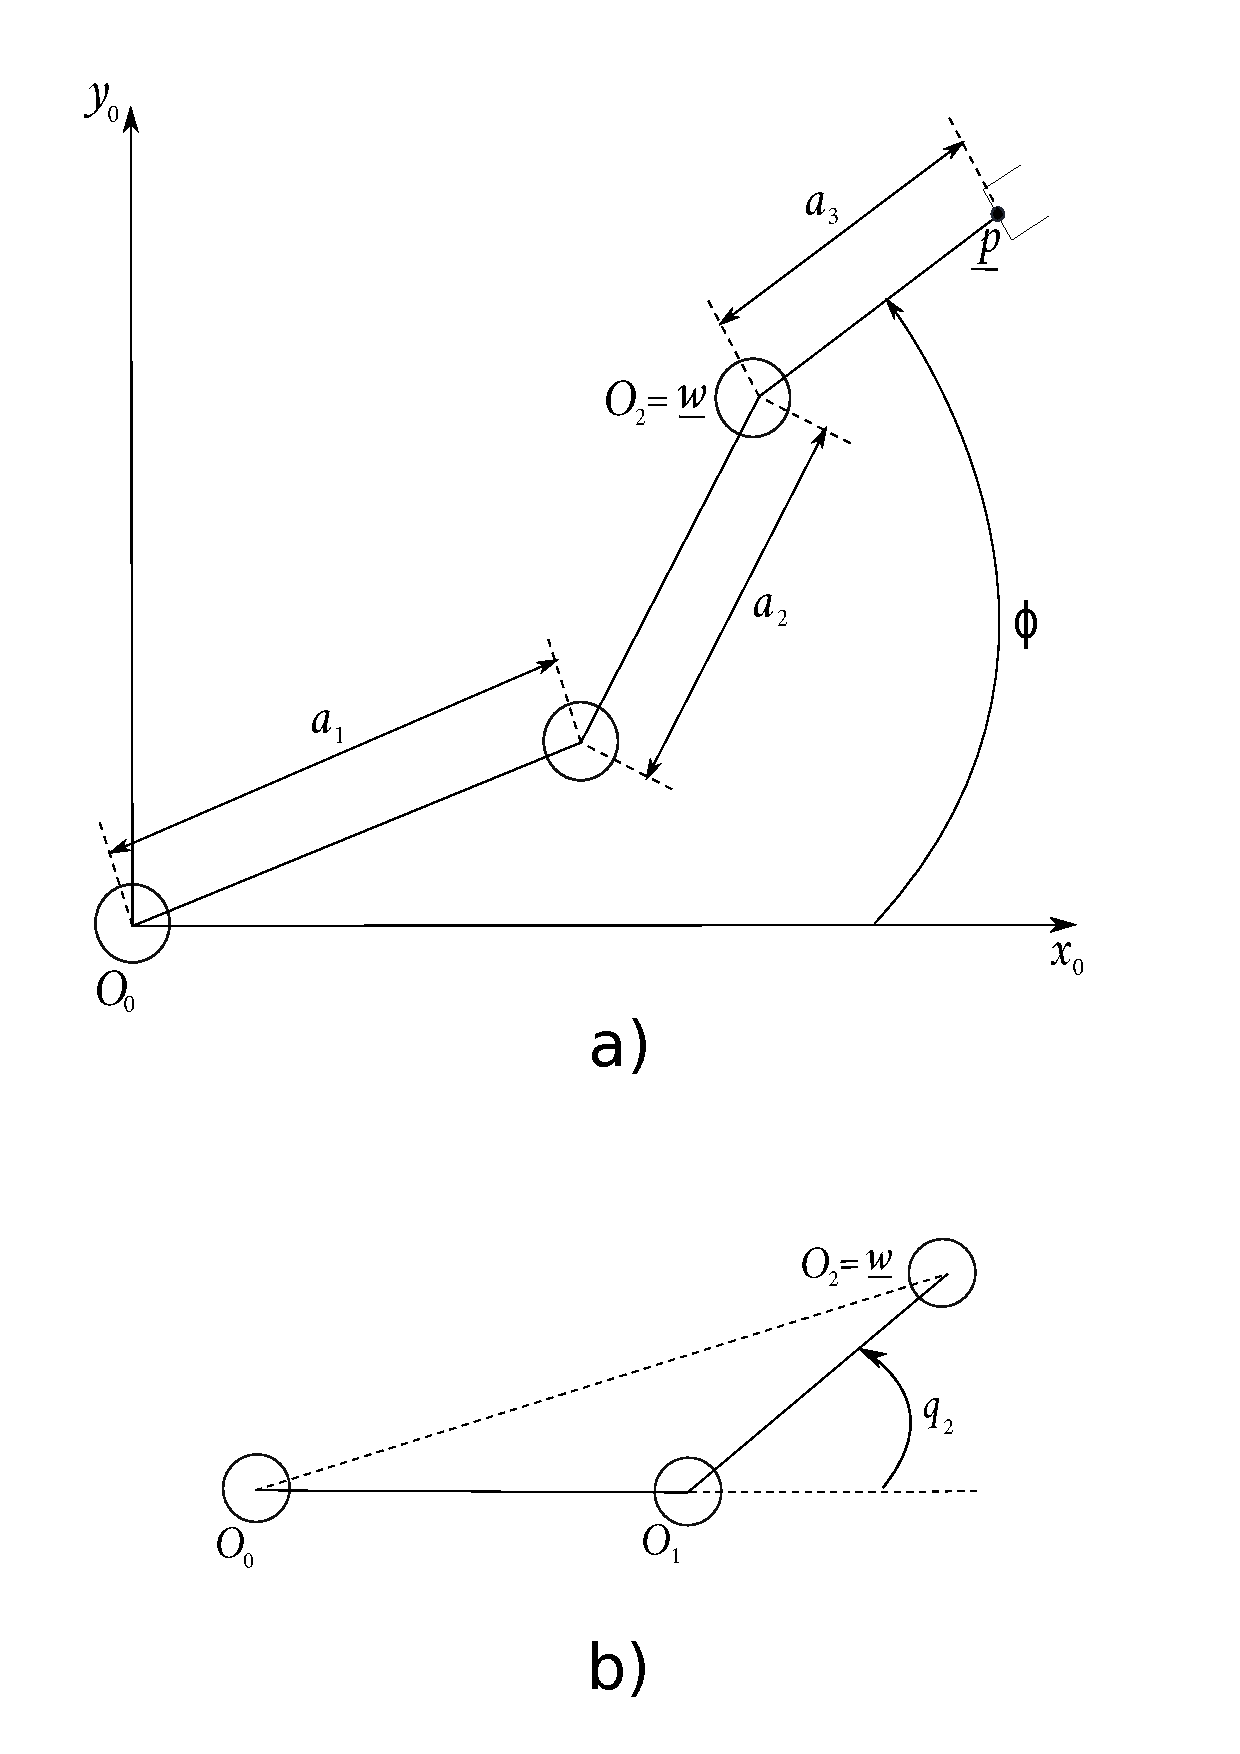
\includegraphics[scale=0.3]{manipolatoreInverso3RGeometria.pdf}
\captionof{figure}{a) Geometria del manipolatore 3R b) Triangolo $OO_1\underline{w}$ }
\end{center}

Quindi, abbiamo la seguente espressione per $\underline{O_2} = \underline{w}$:
\begin{equation*}
	\underline{w} = \underline{p} - a_3\,\underline{i_3} = \underline{p}-a_3
	\begin{bmatrix}
		C_{\phi} \\
		S_{\phi} \\
		0 \\
	\end{bmatrix}
\end{equation*}

Per calcolare $q_1$ e $q_2$ procediamo risolvendo il problema $KIN$ per trovare $\underline{x}$:

\begin{equation*}
	KIN:
	\begin{cases}
		p_x = a_1C_1 + a_2C_{12} + a_3C_{123} \\
		p_y = a_1S_1 + a_2S_{12} + a_3S_{123} \\
		\phi = q_1 + q_2 + q_3 \\
		con \; C_{123} = C_{\phi} \; e \; S_{123} = S_{\phi} \\
	\end{cases} \quad\Rightarrow\quad \underline{x} = 
	\begin{bmatrix}
		p_x \\
		p_y \\
		\phi \\
	\end{bmatrix}
\end{equation*}

quindi otteniamo:
\begin{equation} \label{wx_wy}
	\begin{cases}
		w_x = p_x - a_3C_{\phi} = a_1C_1 + a_2C_{12} \\
		w_y = p_y - a_3S_{\phi} = a_1S_1 + a_2S_{12} \\
	\end{cases}
\end{equation}
A questo punto, per trovare $q_1$ e $q_2$ possiamo procedere per via \emph{algebrica} o per via \emph{geometrica}.

\paragraph{}
Procediamo per via geometrica utilizzando il \emph{teorema di Carnot} per il triangolo in figura 3.3b:
\begin{equation}
	\overline{Ow}^2 = (a_1)^2 + (a_2)^2 - 2a_1a_2\,\cos(\pi - q_2)
\end{equation}

e otteniamo,
\begin{equation*}
	w_x^2 + w_y^2 = (a_1)^2 + (a_2)^2 + 2a_1a_2\,\cos(q_2)
\end{equation*}

pertanto,
\begin{equation*}
	\Rightarrow \quad 
	\cos(q_2) = \dfrac{w_x^2 + w_y^2 - (a_1)^2 - (a_2)^2}{2a_1a_2}
\end{equation*}

esistono due rami di soluzione,
\begin{align}
	q_2 = atan_2(\sqrt{1-C_2^2}, C_2) \\
	q_2 = atan_2(-\sqrt{1-C_2^2}, C_2)
\end{align}
abbiamo trovato la coordinata di giunto $q_2$.

\paragraph{}
Per trovare le altre coordinate di giunto riprendiamo la \eqref{wx_wy} e considerando $C_{12} = \cos(q_1 + q_2) = C_1C_2 - S_1S_2$ e $S_{12} = \sin(q_1 + q_2) = S_1C_2 + S_2C_1$,
\begin{equation}
	\begin{cases}
		w_x = p_x - a_3C_{\phi} = a_1C_1 + a_2(C_1C_2 - S_1S_2) \\
		w_y = p_y - a_3S_{\phi} = a_1S_1 + a_2(S_1C_2 + S_2C_1) \\
	\end{cases}
\end{equation}

in questo sistema lineare le incognite sono solo $S_1$ e $C_1$ e pertanto scrivo:
\begin{equation}
	\begin{bmatrix}
		w_x \\
		w_y \\
	\end{bmatrix}
	=
	\begin{bmatrix}
		a_1 + a_2C_2 & -a_2S_2 \\
		a_2S_2 & a_1 + a_2C_2 \\ 
	\end{bmatrix}
	\cdot
	\begin{bmatrix}
		C_1 = \cos(q_1) \\
		S_1 = \sin(q_1) \\
	\end{bmatrix}
\end{equation}

e ottengo,
\begin{equation}
	\begin{cases}
		q_1 = atan_2(S_1, C_1) \\
		q_2 = equazione\;(3.6) \\
		q_3 = \phi - q_1 - q_2 \\
	\end{cases}
\end{equation}
	
\subsubsection{Robot planare 4R}
Se abbiamo un robot planare 4R, è possibile soddisfare la specifica posizionale e quella di orientazione e le soluzioni possibili saranno $\infty$, infatti il 4R è cinematicamente ridondante (nel piano) perchè dato un punto $\underline{p}$, possiamo raggiungerlo in infiniti modi (infinite configurazioni).

\begin{center}
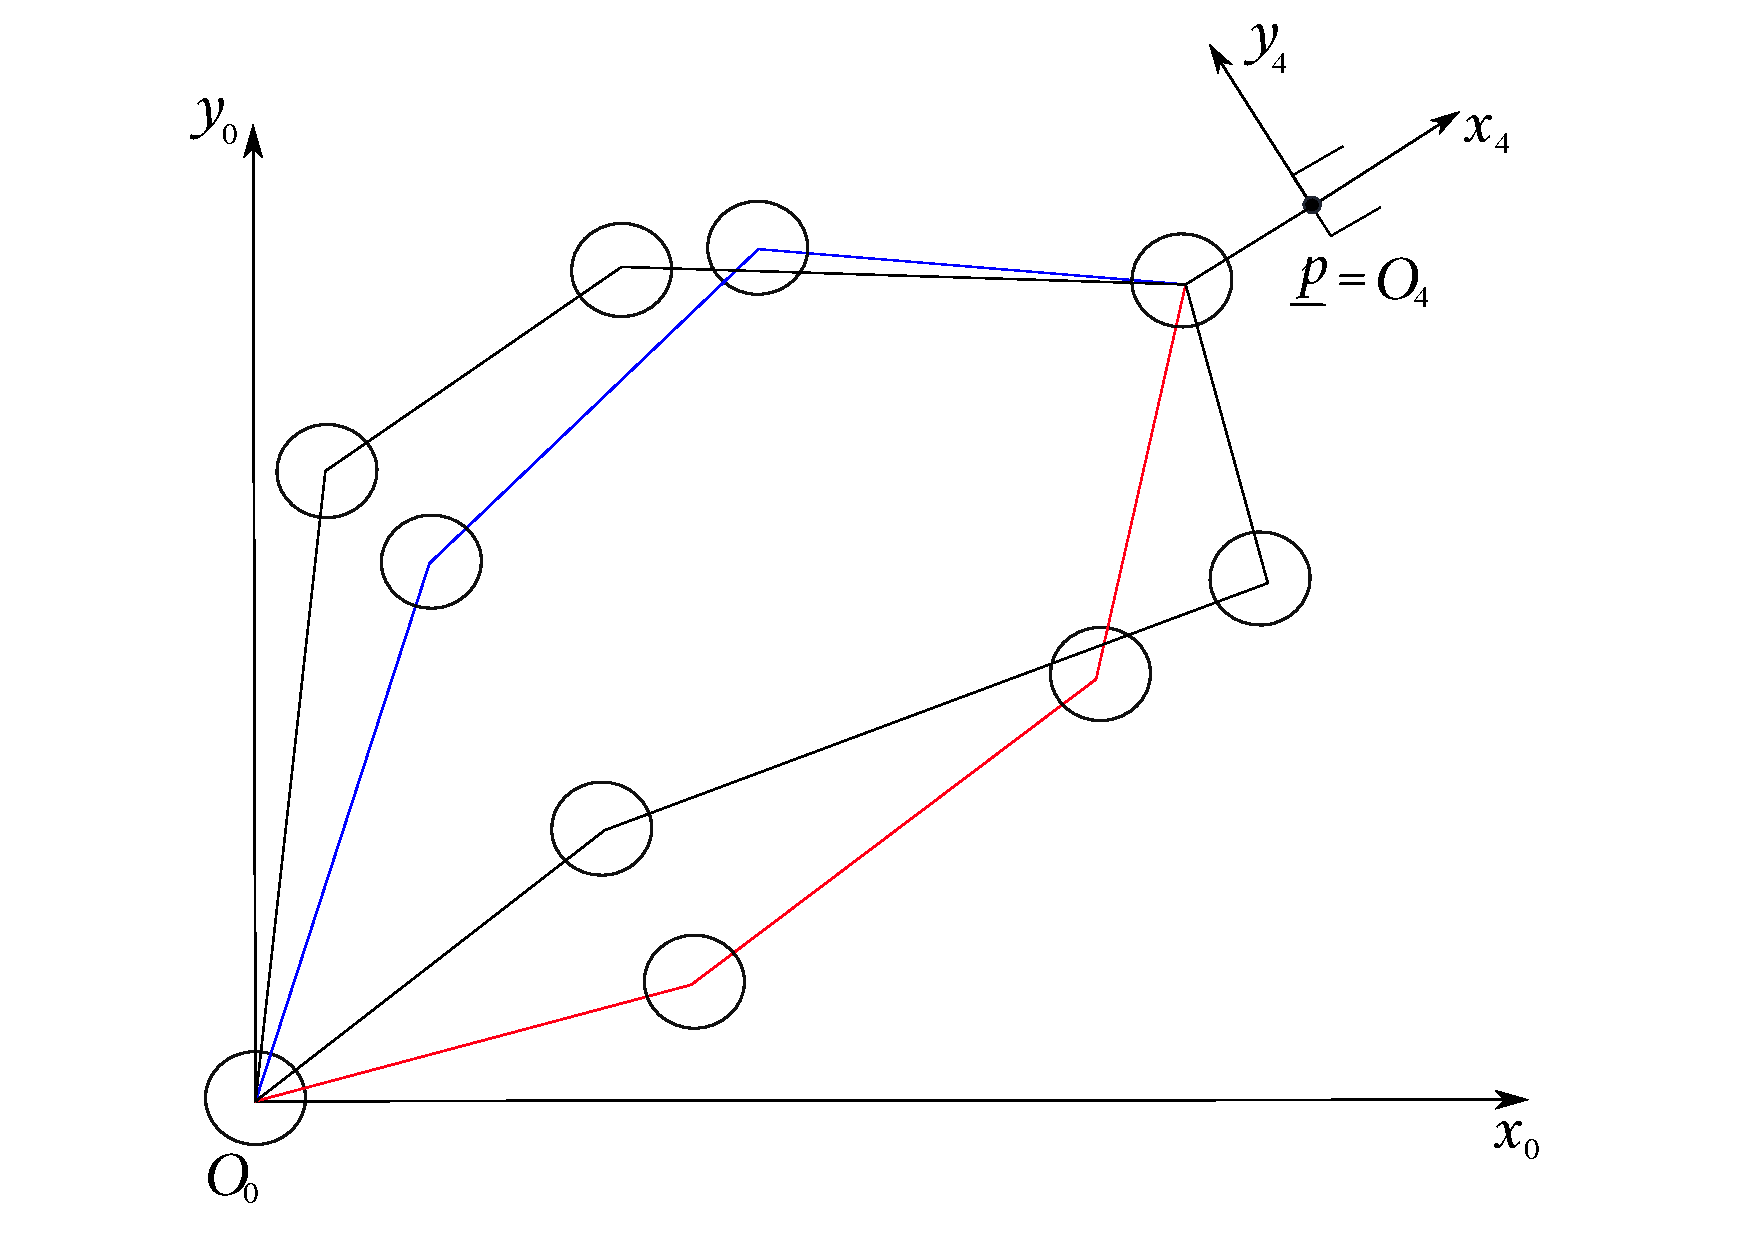
\includegraphics[scale=0.3]{manipolatoreInverso4R.pdf}
\captionof{figure}{Possibili configurazioni del manipolatore 4R}
\end{center}

\section{$KIN^{-1}$ di manipolatori con polso sferico}
Adesso esaminiamo un manipolatore spaziale. Pieper dimostrò che:
\paragraph{}
\emph{Per ogni manipolatore a 6 DOF in cui esistono tre giunti adiacenti con assi che si intersecano in un unico punto, allora la soluzione del problema cinematico inverso esiste in forma chiusa.}
\paragraph{}
Un particolare tipo di struttura con tre assi di giunti adiacenti che si intersecano in un punto è il giunto sferico (polso) di tipo roll-pitch-roll mostrato in figura.

\begin{center}
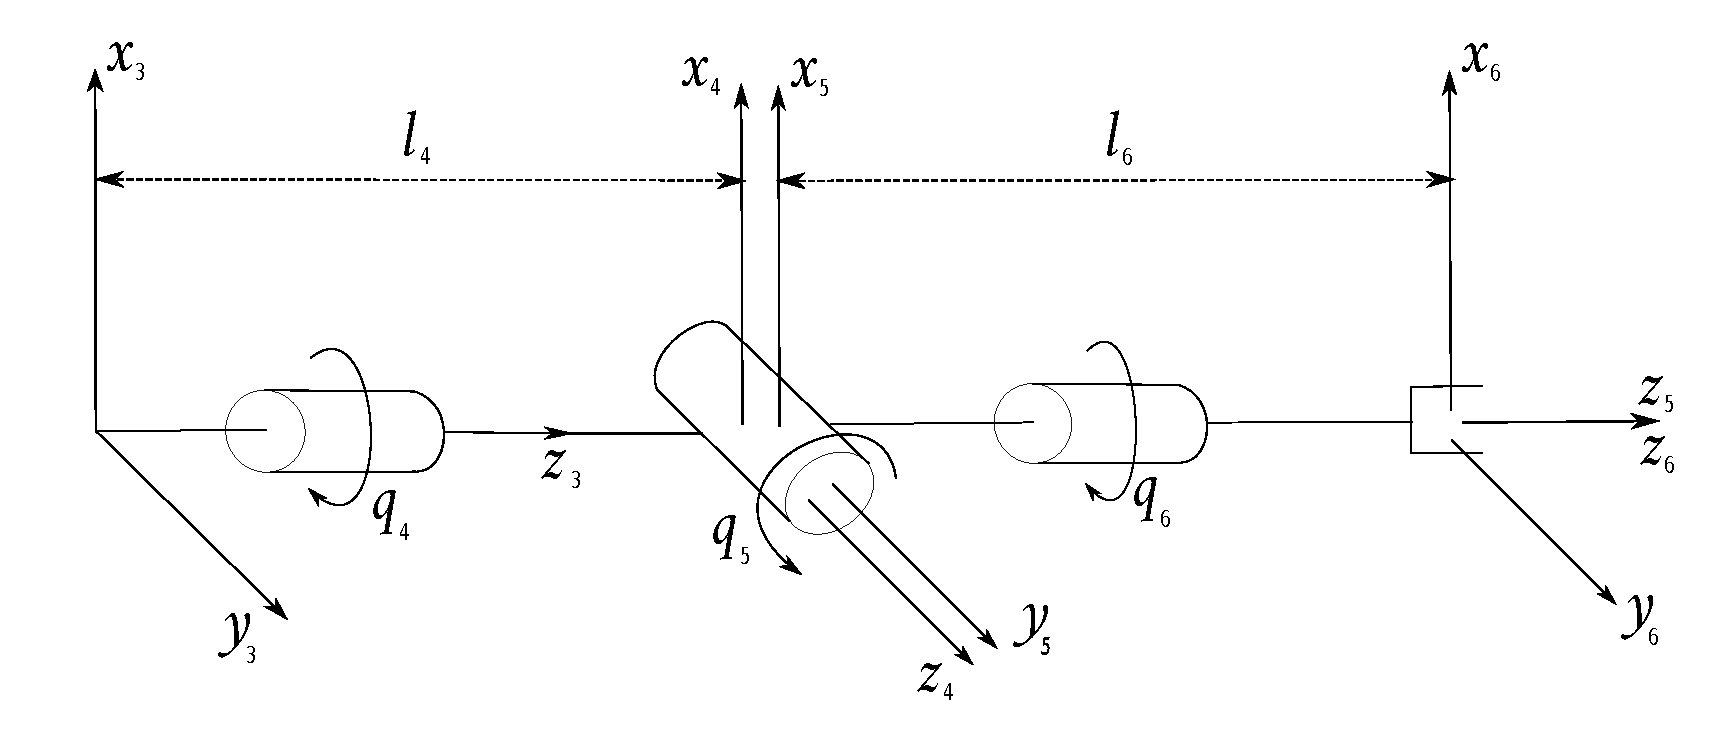
\includegraphics[scale=0.225]{polsoSfericoSingolare.pdf}
\captionof{figure}{Configurazione Singolare del polso $z_5 \parallel z_6$} 
\end{center}

\paragraph{}
Il manipolatore completo a 6 DOF (figura $2.8$) composto da una struttura di manipolazione a 3 DOF più un polso sferico anch'esso a 3 DOF soddisfa ancora la \emph{condizione di Pieper}. 

Possiamo definire un \emph{"metodo generale per $KIN^{-1}$ di manipolatori con polso sferico"}. Iniziamo scrivendo i \emph{dati del problema}:
\begin{itemize}
	\item $\underline{p} = \underline{O_6}$ 
	\item $R = R_6^0$
\end{itemize}

\paragraph{}
Possiamo suddividere il problema a 6 DOF in due sottoproblemi più semplici a 3 DOF ciascuno. Una volta nota la posizione e l'orientazione desiderata dell'organo terminale, la posizione del \emph{centro del polso} $\underline{w}$ è calcolabile come segue:
\begin{equation} \label{w_polso}
	\underline{w} = \underline{p} - l_6\,\underline{k_5}
\end{equation}

e la posizione del centro del polso dipende solo dalle coordinate dei primi tre giunti del robot:
\begin{equation} \label{funzione_w}
	\underline{w} = \underline{w}(q_1, q_2, q_3)
\end{equation}
notiamo che la \eqref{w_polso} rappresenta il calcolo di $\underline{w}$ in funzione dei dati del problema e che $\underline{k_5} = \underline{k_6}$ è la terza colonna di $R = R_6^0$

\paragraph{}
Quindi si può risolvere in modo agevole il problema della cinematica inversa della struttura di manipolazione, ottenendo $q_1$, $q_2$, $q_3$ dalla \eqref{funzione_w}, scriviamo i passi:
\begin{enumerate}
	\item[1)] Calcolare $q_1$, $q_2$, $q_3$ tali che: $\underline{w}(q_1, q_2, q_3) = \underline{p} - l_6\,\underline{k_5} = \underline{w}_{\,des}$
	\item[2)] Calcolare $q_4$, $q_5$, $q_6$ tali che: $R_3^0(q_1, q_2, q_3) \cdot R_6^3(q_4, q_5, q_6) = R$
	\begin{enumerate}
		\item[2.1)] noti $q_1$, $q_2$, $q_3$ dalla $KIN^{-1}$, calcolo $R_3^0(q_1, q_2, q_3)$
		\item[2.2)] avendo calcolato $R_3^0$ e avendo $R$ noto (come dato del problema) calcolo $R_3^0\,R_6^0 = R \Rightarrow R_6^3 = (R_3^0)^T\,R$
		\item[2.3)] avendo calcolato $R_6^3$ posso calcolare $R_6^3 = R_6^3(q_4, q_5, q_6)$ per trovare $q_4$, $q_5$, $q_6$ è possibile utilizzare le formule di inversione della \emph{matrice di Eulero}, infatti, posso scrivere:
		\begin{equation}
			R_6^3(q_4, q_5, q_6) = R_{zyz}(\varphi, \theta, \psi) \quad con 
			\begin{cases}
				\varphi = q_4 \\
				\theta = q_5 \\
				\psi = q_6 \\
			\end{cases}
		\end{equation}
	\end{enumerate}
\end{enumerate}